\documentclass[a4paper,10pt,twoside]{article}

\usepackage[top=1in, bottom=1in, left=1in, right=1in]{geometry}
\usepackage[utf8]{inputenc}
\usepackage[spanish,es-ucroman,es-noquoting]{babel}
\usepackage{setspace}
\usepackage{fancyhdr}
\usepackage{lastpage}
\usepackage{amsmath}
\usepackage{amsfonts}
\usepackage{verbatim}
\usepackage{float}
\usepackage{graphicx}
\usepackage{subcaption}
\usepackage{algorithmic}
\usepackage{amssymb}
\usepackage{url}
\usepackage{moreverb}


% Evita que el documento se estire verticalmente para ocupar
% el espacio vacío en cada página.
\raggedbottom


%%%%%%%%%% Configuración de Fancyhdr - Inicio %%%%%%%%%%
\pagestyle{fancy}
\thispagestyle{fancy}
\lhead{Trabajo Práctico 2, Organización del Computador II}
\rhead{Capra, Lovisolo, Petaccio}
\renewcommand{\footrulewidth}{0.4pt}
\cfoot{\thepage /\pageref{LastPage}}

\fancypagestyle{caratula} {
   \fancyhf{}
   \cfoot{\thepage /\pageref{LastPage}}
   \renewcommand{\headrulewidth}{0pt}
   \renewcommand{\footrulewidth}{0pt}
}
%%%%%%%%%% Configuración de Fancyhdr - Fin %%%%%%%%%%

\begin{document}


%%%%%%%%%%%%%%%%%%%%%%%%%%%%%%%%%%%%%%%%%%%%%%%%%%%%%%%%%%%%%%%%%%%%%%%%%%%%%%%
%% Carátula                                                                  %%
%%%%%%%%%%%%%%%%%%%%%%%%%%%%%%%%%%%%%%%%%%%%%%%%%%%%%%%%%%%%%%%%%%%%%%%%%%%%%%%


\thispagestyle{caratula}

\begin{center}


\includegraphics[height=2cm]{DC.png} 
\hfill

\includegraphics[height=2cm]{UBA.jpg} 

\vspace{2cm}

Departamento de Computación,\\
Facultad de Ciencias Exactas y Naturales,\\
Universidad de Buenos Aires

\vspace{2cm}

\begin{spacing}{1}
\begin{Huge}

Reconocimiento de Dígitos Manuscritos\\
con la Descomposición en Valores Singulares

\end{Huge}
\end{spacing}

\vspace{2cm}

Trabajo Práctico 1, \\
Métodos Numéricos, \\
Primer Cuatrimestre de 2013

\vspace{3cm}

\begin{tabular}{|c|c|c|}
\hline
Apellido y Nombre & LU & E-mail\\
\hline
María Candela Capra Coarasa & 234/11 & canduh\_27@hotmail.com\\
Leandro Lovisolo            & 645/11 & leandro@leandro.me\\
Lautaro José Petaccio       & 443/11 & lausuper@gmail.com\\
\hline
\end{tabular}

\end{center}

\vspace{3cm}

\textbf{Resumen:} \\
Se implementa un método de reconocimiento de dígitos manuscritos basado en la descomposición en valores singulares, y se analizan empíricamente los parámetros principales del método.

\textbf{Palabras clave:}
OCR, dígitos manuscritos, reconocimiento, SVD, algoritmo QR.

\newpage


%%%%%%%%%%%%%%%%%%%%%%%%%%%%%%%%%%%%%%%%%%%%%%%%%%%%%%%%%%%%%%%%%%%%%%%%%%%%%%%
%% Índice                                                                    %%
%%%%%%%%%%%%%%%%%%%%%%%%%%%%%%%%%%%%%%%%%%%%%%%%%%%%%%%%%%%%%%%%%%%%%%%%%%%%%%%


\tableofcontents

\newpage


%%%%%%%%%%%%%%%%%%%%%%%%%%%%%%%%%%%%%%%%%%%%%%%%%%%%%%%%%%%%%%%%%%%%%%%%%%%%%%%
%% Introducción Teórica                                                      %%
%%%%%%%%%%%%%%%%%%%%%%%%%%%%%%%%%%%%%%%%%%%%%%%%%%%%%%%%%%%%%%%%%%%%%%%%%%%%%%%


\section{Introducción Teórica}

\subsection{Conceptos}

\subsubsection{Media}
La media ($\bar{x} = \frac{1}{n} \sum_{i=1}^{n} x_i$) es un promedio estándard comunmente relacionado con la distribución probabilística Normal. El promedio es la esperanza de esta distribución.

En nuestro caso se utilizará la media de las columnas de la matriz que utilizaremos para el método OCR.

\subsubsection{Varianza}
La varianza es una medida de dispersión definida como la esperanza del cuadrado de la desviación de dicha variable respecto a su media.

En nuestro caso, debido a que utilizaremos una matríz para el método de OCR, el cálculo de la varianza será: $\sigma x_i = \frac{1}{n-1} \sum_{j=1}^{n} (x_i^{(j)} - \bar{x}_i)^2$.

\subsubsection{Matriz de covarianza}
La covarianza es un valor que indica el grado de variación conjunta de dos variables aleatorias, su ecuación es la siguiente:

 $\sigma x_k,x_j = \frac{1}{n-1} \sum{i=1}^{n} (x_k^{(i)} - \bar{x}_k)(x_j^{(i)} - \bar{x}_j) = \frac{1}{n-1}(x_k - \bar{x}_k)^{t}(x_j - \bar{x}_j)$

Dadas las imágenes utilizadas para el caso en formas de fila en la matriz (la llamaremos matriz A), la matriz de covarianza se construye de la siguiente forma:

$Mx = \frac{1}{n-1} X^{t}X = 
 \begin{pmatrix}
  \sigma x_1,x_1 & \sigma x_1,x_2 & \cdots & \sigma x_1,x_n \\
  \sigma x_2,x_1 & \sigma x_2,x_2 & \cdots & \sigma x_2,x_n \\
  \vdots  & \vdots  & \ddots & \vdots  \\
  \sigma x_n,x_1 & \sigma x_n,x_2 & \cdots & \sigma x_n,x_n \\
 \end{pmatrix}
$
\\
Siendo la matriz $X = 
 \begin{pmatrix}
  a_{1,1} - \bar{a_1} & a_{1,2} - \bar{a_2} & \cdots & a_{1,m} - \bar{a_m} \\
  a_{2,1} - \bar{a_1} & a_{2,2} - \bar{a_2} & \cdots & a_{2,m} - \bar{a_m} \\
  \vdots  & \vdots  & \ddots & \vdots  \\
  a_{n,1} - \bar{a_1} & a_{n,2} - \bar{a_2} & \cdots & a_{n,m} - \bar{a_m} \\
 \end{pmatrix}
$

Se utiliza la matríz de covarianza para poder realizar luego una reducción de la redundancia en la información (reduciendo la covarianza) obteniendo los datos impresindibles y necesarios para la aplicación del método elegido de OCR.

La matriz de covarianza cuenta con la propiedad de ser simétrica, dado que $X^{t}X = (X^{t}X)^{t} = (X^{t}X^{t^{t}}) = X^{t}X$ permitiendo la utilización de métodos como QR para conseguir sus autovectores y autovalores.

\subsubsection{Diagonalización de la matriz}
\textbf{Teorema:}
Si $\mathnormal{B} \in \mathbb{R}^{nxn}$ es simétrica, entonces existe una base ortonormal de autovectores ${v_1,..,v_n}$ asociados a autovalores $\lambda_1 .. \lambda_n$.

Como la matriz de covarianzas es simétrica, según el teorema, esta tiene una base ortonormal de autovectores por lo que es diagonalizable y es posible expresarse de la forma $Mx = VDV^{t} = U \Sigma V^{t}$ (descomposición SVD de la matriz).

\subsubsection{Método de diagonalización QR}
Utilizando la propiedad de que las matrices simétricas son diagonalizables, se construye el siguiente algoritmo utilizando algún método de factorización QR.

\begin{algorithmic}
  \WHILE{Cota elegida}
    \STATE FactorizaciónQR($A_k$) $\rightarrow Q_k R_k$
    \STATE $A_{k+1} \leftarrow R_k Q_k$
  \ENDWHILE
\end{algorithmic}


%%%%%%%%%%%%%%%%%%%%%%%%%%%%%%%%%%%%%%%%%%%%%%%%%%%%%%%%%%%%%%%%%%%%%%%%%%%%%%%
%% Desarrollo                                                                %%
%%%%%%%%%%%%%%%%%%%%%%%%%%%%%%%%%%%%%%%%%%%%%%%%%%%%%%%%%%%%%%%%%%%%%%%%%%%%%%%


\section{Desarrollo}
Se realizó la implementación en C++ utilizando la clase Matriz utilizada anteriormente en el TP2 de la materia. A esta se le agregaron entre otros, los métodos de House Holder y Givens para la realización de la diagonalización mediante el método QR de la matriz de covarianza.

La implementación de Givens resultó ser demasiado lenta (debido a la naturaleza de la matriz Mx) a comparación de la de House Holder a la hora de diagonalizar por lo que la diagonalización de la matriz de covarianza fué realizada mediante House Holder.

El criterio de parada o cota utilizada para el método de diagonalización fue la suma de los elementos por debajo de la diagonal.

Una vez obtenida la matriz de autovectores mediante el método de diagonalización, se reordenaron los autovectores y autovalores asociados de forma decreciente en valor absoluto.

El método elegido para la detección de dígitos fué el siguiente:
\begin{enumerate}
\item Del set de entrenamiento, se filtró las imágenes (filas de la matríz de imágenes MISNT) según cáda dígito (0-9) y se armó nuevas matrices con estas.

\item A cada matríz con las imágenes de los dígitos filtrados se les aplicó $TC(X_{0..9})$ dónde $TC(X) = V^{t} * X^{t}$ realizando una transformación de todas las imágenes en la matriz de cáda dígito.

$V^{t}$ es reducida según el valor de columnas k elegidas para comprobar la efectividad del método SVD ante la eliminación de la redundancia.

\item Se creó una nueva matriz a la que llamaremos "matriz de medias" la cuál contiene en sus 10 filas, las medias de las columnas de las matrices filtradas por dígitos y transformadas.

\item Dado el set de pruebas, se procedió a transformar las imágenes (filas de la matriz obtenida para tests de MNST) utilizando $TC()$ , se les calculó su media y se la comparó con las filas de la matriz de medias con el objetivo de encontrar la fila que produzca el menor error cuadrático entre las diferentes medias y la media obtenida, pudiendo así elegir el dígito correspondiente a la fila que tuviera menor error cuadrático.
\end{enumerate}

Este experimento se replicó con diferentes cantidades de imágenes de entrenamiento, con diferentes k's para el cálculo de $TC()$ y con diferentes cotas a la hora del cálculo de autovalores y autovectores.


%%%%%%%%%%%%%%%%%%%%%%%%%%%%%%%%%%%%%%%%%%%%%%%%%%%%%%%%%%%%%%%%%%%%%%%%%%%%%%%
%% Resultados                                                                %%
%%%%%%%%%%%%%%%%%%%%%%%%%%%%%%%%%%%%%%%%%%%%%%%%%%%%%%%%%%%%%%%%%%%%%%%%%%%%%%%


\section{Resultados}

\begin{figure}[H]
  \centering
  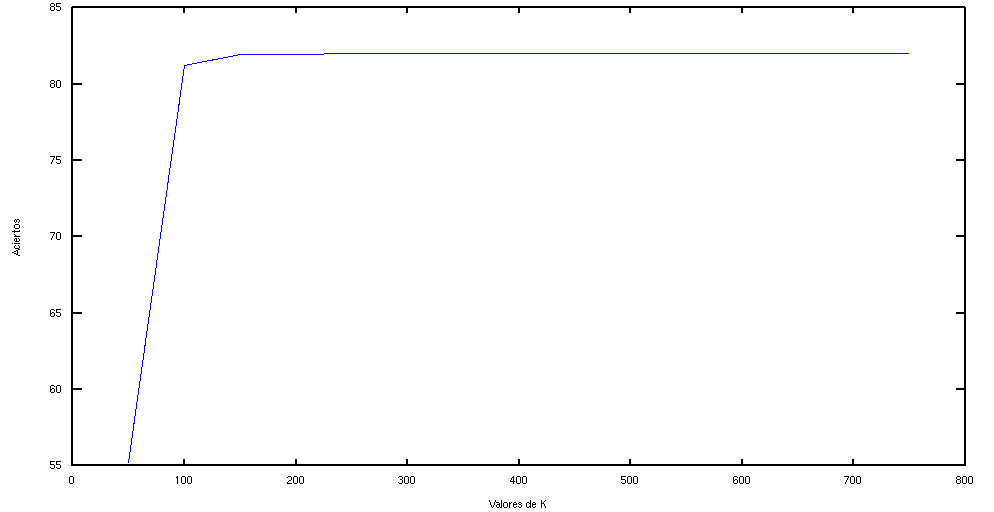
\includegraphics[width=15cm]{aciertosVsK.png}
  \caption{Resultados con diferentes K utilizando cota 1000 para generar V}
\end{figure}

\begin{figure}[H]
  \centering
  % GNUPLOT: LaTeX picture with Postscript
\begingroup
  \makeatletter
  \providecommand\color[2][]{%
    \GenericError{(gnuplot) \space\space\space\@spaces}{%
      Package color not loaded in conjunction with
      terminal option `colourtext'%
    }{See the gnuplot documentation for explanation.%
    }{Either use 'blacktext' in gnuplot or load the package
      color.sty in LaTeX.}%
    \renewcommand\color[2][]{}%
  }%
  \providecommand\includegraphics[2][]{%
    \GenericError{(gnuplot) \space\space\space\@spaces}{%
      Package graphicx or graphics not loaded%
    }{See the gnuplot documentation for explanation.%
    }{The gnuplot epslatex terminal needs graphicx.sty or graphics.sty.}%
    \renewcommand\includegraphics[2][]{}%
  }%
  \providecommand\rotatebox[2]{#2}%
  \@ifundefined{ifGPcolor}{%
    \newif\ifGPcolor
    \GPcolorfalse
  }{}%
  \@ifundefined{ifGPblacktext}{%
    \newif\ifGPblacktext
    \GPblacktexttrue
  }{}%
  % define a \g@addto@macro without @ in the name:
  \let\gplgaddtomacro\g@addto@macro
  % define empty templates for all commands taking text:
  \gdef\gplbacktext{}%
  \gdef\gplfronttext{}%
  \makeatother
  \ifGPblacktext
    % no textcolor at all
    \def\colorrgb#1{}%
    \def\colorgray#1{}%
  \else
    % gray or color?
    \ifGPcolor
      \def\colorrgb#1{\color[rgb]{#1}}%
      \def\colorgray#1{\color[gray]{#1}}%
      \expandafter\def\csname LTw\endcsname{\color{white}}%
      \expandafter\def\csname LTb\endcsname{\color{black}}%
      \expandafter\def\csname LTa\endcsname{\color{black}}%
      \expandafter\def\csname LT0\endcsname{\color[rgb]{1,0,0}}%
      \expandafter\def\csname LT1\endcsname{\color[rgb]{0,1,0}}%
      \expandafter\def\csname LT2\endcsname{\color[rgb]{0,0,1}}%
      \expandafter\def\csname LT3\endcsname{\color[rgb]{1,0,1}}%
      \expandafter\def\csname LT4\endcsname{\color[rgb]{0,1,1}}%
      \expandafter\def\csname LT5\endcsname{\color[rgb]{1,1,0}}%
      \expandafter\def\csname LT6\endcsname{\color[rgb]{0,0,0}}%
      \expandafter\def\csname LT7\endcsname{\color[rgb]{1,0.3,0}}%
      \expandafter\def\csname LT8\endcsname{\color[rgb]{0.5,0.5,0.5}}%
    \else
      % gray
      \def\colorrgb#1{\color{black}}%
      \def\colorgray#1{\color[gray]{#1}}%
      \expandafter\def\csname LTw\endcsname{\color{white}}%
      \expandafter\def\csname LTb\endcsname{\color{black}}%
      \expandafter\def\csname LTa\endcsname{\color{black}}%
      \expandafter\def\csname LT0\endcsname{\color{black}}%
      \expandafter\def\csname LT1\endcsname{\color{black}}%
      \expandafter\def\csname LT2\endcsname{\color{black}}%
      \expandafter\def\csname LT3\endcsname{\color{black}}%
      \expandafter\def\csname LT4\endcsname{\color{black}}%
      \expandafter\def\csname LT5\endcsname{\color{black}}%
      \expandafter\def\csname LT6\endcsname{\color{black}}%
      \expandafter\def\csname LT7\endcsname{\color{black}}%
      \expandafter\def\csname LT8\endcsname{\color{black}}%
    \fi
  \fi
  \setlength{\unitlength}{0.0500bp}%
  \begin{picture}(7678.00,5280.00)%
    \gplgaddtomacro\gplbacktext{%
      \colorrgb{0.00,0.00,0.00}%
      \put(620,640){\makebox(0,0)[r]{\strut{}30}}%
      \colorrgb{0.00,0.00,0.00}%
      \put(620,1313){\makebox(0,0)[r]{\strut{}40}}%
      \colorrgb{0.00,0.00,0.00}%
      \put(620,1986){\makebox(0,0)[r]{\strut{}50}}%
      \colorrgb{0.00,0.00,0.00}%
      \put(620,2660){\makebox(0,0)[r]{\strut{}60}}%
      \colorrgb{0.00,0.00,0.00}%
      \put(620,3333){\makebox(0,0)[r]{\strut{}70}}%
      \colorrgb{0.00,0.00,0.00}%
      \put(620,4006){\makebox(0,0)[r]{\strut{}80}}%
      \colorrgb{0.00,0.00,0.00}%
      \put(620,4679){\makebox(0,0)[r]{\strut{}90}}%
      \colorrgb{0.00,0.00,0.00}%
      \put(740,440){\makebox(0,0){\strut{}0}}%
      \colorrgb{0.00,0.00,0.00}%
      \put(2055,440){\makebox(0,0){\strut{}20}}%
      \colorrgb{0.00,0.00,0.00}%
      \put(3371,440){\makebox(0,0){\strut{}40}}%
      \colorrgb{0.00,0.00,0.00}%
      \put(4686,440){\makebox(0,0){\strut{}60}}%
      \colorrgb{0.00,0.00,0.00}%
      \put(6002,440){\makebox(0,0){\strut{}80}}%
      \colorrgb{0.00,0.00,0.00}%
      \put(7317,440){\makebox(0,0){\strut{}100}}%
      \colorrgb{0.00,0.00,0.00}%
      \put(160,2659){\rotatebox{90}{\makebox(0,0){\strut{}Aciertos [\%]}}}%
      \colorrgb{0.00,0.00,0.00}%
      \put(4028,140){\makebox(0,0){\strut{}$k$}}%
      \csname LTb\endcsname%
      \put(4028,4979){\makebox(0,0){\strut{}Tasa de aciertos en función de cantidad de coeficientes principales $k$}}%
    }%
    \gplgaddtomacro\gplfronttext{%
    }%
    \gplbacktext
    \put(0,0){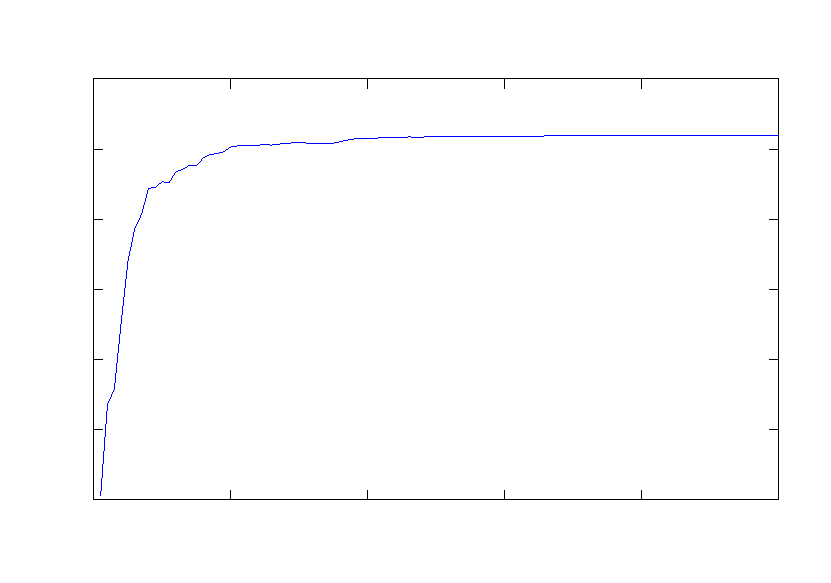
\includegraphics{tasas-vs-k}}%
    \gplfronttext
  \end{picture}%
\endgroup

  \caption{Tasa de aciertos en función de k}
\end{figure}


%%%%%%%%%%%%%%%%%%%%%%%%%%%%%%%%%%%%%%%%%%%%%%%%%%%%%%%%%%%%%%%%%%%%%%%%%%%%%%%
%% Discusión                                                                 %%
%%%%%%%%%%%%%%%%%%%%%%%%%%%%%%%%%%%%%%%%%%%%%%%%%%%%%%%%%%%%%%%%%%%%%%%%%%%%%%%


\section{Discusión}


%%%%%%%%%%%%%%%%%%%%%%%%%%%%%%%%%%%%%%%%%%%%%%%%%%%%%%%%%%%%%%%%%%%%%%%%%%%%%%%
%% Conclusiones                                                              %%
%%%%%%%%%%%%%%%%%%%%%%%%%%%%%%%%%%%%%%%%%%%%%%%%%%%%%%%%%%%%%%%%%%%%%%%%%%%%%%%


\section{Conclusiones}


%%%%%%%%%%%%%%%%%%%%%%%%%%%%%%%%%%%%%%%%%%%%%%%%%%%%%%%%%%%%%%%%%%%%%%%%%%%%%%%
%% Apéndice A: Enunciado del Trabajo Práctico                                %%
%%%%%%%%%%%%%%%%%%%%%%%%%%%%%%%%%%%%%%%%%%%%%%%%%%%%%%%%%%%%%%%%%%%%%%%%%%%%%%%


\newpage

\section{Apéndice A: Enunciado del Trabajo Práctico}

{\bf Introducci\'on}\\

El reconocimiento \'optico de caracteres (OCR, por sus siglas en ingl\'es) es el proceso por el cual se traducen o convierten im\'agenes de d\'igitos o caracteres (sean \'estos manuscritos o de alguna tipograf\'ia especial) a un formato representable en nuestra computadora (por ejemplo, ASCII). Esta tarea puede ser m\'as sencilla (por ejemplo, cuando tratamos de determinar el texto escrito en una versi\'on escaneada a buena resoluci\'on de un libro) o tornarse casi imposible (recetas indescifrables de m\'edicos, algunos parciales manuscritos de alumnos de m\'etodos num\'ericos, etc).

El objetivo del trabajo pr\'actico es implementar un m\'etodo de reconocimiento de d\'igitos manuscritos basado en la descomposici\'on en valores singulares, y analizar emp\'iricamente los par\'ametros principales del m\'etodo.

Como instancias de entrenamiento, se tiene un conjunto de $n$ im\'agenes de d\'igitos ma\-nus\-cri\-tos en escala de grises del mismo tama\~no y resoluci\'on (varias im\'agenes de cada d\'igito). Cada una de estas im\'agenes sabemos a qu\'e d\'igito se corresponde.
En este trabajo consideraremos la popular base de datos MNIST, utilizada como referencia en esta \'area de investigaci\'on\footnote{\texttt{http://yann.lecun.com/exdb/mnist/}}. 

Para $i = 1,\ldots, n$, sea $x_i \in \real^{m}$ la $i$-\'esima imagen de nuestra base de datos almacenada por filas en un vector, y sea $\mu = (x_1 + \ldots + x_n)/n$ el promedio de las im\'agenes. Definimos $X\in\real^{n\times m}$ como la matriz que contiene en la $i$-\'esima fila al vector $(x_i - \mu)^{t}/\sqrt{n-1}$, y $$X=U \Sigma V^t$$ a su descomposici\'on en valores singulares, con $U\in\real^{n\times n}$ y $V\in\real^{m\times m}$ matrices ortogonales, y $\Sigma\in\real^{n\times m}$ la matriz diagonal conteniendo en la posici\'on $(i,i)$ al $i$-\'esimo valor singular $\sigma_i$.
Siendo $v_i$ la columna $i$ de $V$, definimos para $i = 1,\ldots,n$ la \textsl{transformaci\'on caracter\'istica} del d\'igito $x_{i}$ como el vector $\mathbf{tc}(x_i) = (v_1^t\, x_i, v_2^t\, x_i,\ldots,v_k^t\, x_i) \in\real^k$, donde $k \in\{1,\ldots,m\}$ es un par\'ametro de la implementaci\'on. Este proceso corresponde a extraer las $k$ primeras \textit{componentes principales} de cada imagen. La intenci\'on es que $\mathbf{tc}(x_i)$ resuma la informaci\'on m\'as relevante de la imagen, descartando los detalles o las zonas que no aportan rasgos distintivos.

Dada una nueva imagen $x$ de un d\'igito manuscrito, que no se encuentra en el conjunto inicial de im\'agenes de entrenamiento, el problema de reconocimiento consiste en determinar a qu\'e d\'igito corresponde. Para esto, se calcula $\mathbf{tc}(x)$ y se compara con $\mathbf{tc}(x_i)$, para $i = 1,\ldots, n$. \\

{\bf Enunciado}\\

Se pide implementar un programa que lea desde archivos las im\'agenes de entrenamiento de distintos d\'igitos manuscritos y que, utilizando la descomposici\'on en valores singulares, se calcule la transformaci\'on caracter\'istica de acuerdo con la descripci\'on anterior. Para ello se deber\'a implementar alg\'un m\'etodo de estimaci\'on de autovalores/autovectores. Dada una nueva imagen de un d\'igito manuscrito, el programa deber\'a determinar a qu\'e d\'igito co\-rres\-pon\-de.
El formato de los archivos de entrada y salida queda a elecci\'on del grupo. Si no usan un entorno de desarrollo que incluya bibliotecas para la lectura de archivos de im\'agenes, sugerimos que utilicen im\'agenes en formato \textsc{Raw}. 

Se deber\'an realizar experimentos para medir la efectividad del reconocimiento, analizando tanto la influencia de la cantidad $k$ de componentes principales seleccionadas como la influencia de la precisi\'on en el c\'alculo de los autovalores.\\

{\bf Fecha de entrega} 

\begin{itemize}
\item \textsl{Formato electr\'onico:} viernes 21 de junio de 2013, \underline{hasta las 23:59 hs.}, enviando el trabajo (informe+c\'odigo) a \texttt{metnum.lab@gmail.com}. El subject del email debe comenzar con el texto \verb|[TP3]| seguido de la lista de apellidos de los integrantes del grupo. 
\item \textsl{Formato f\'isico:} lunes 24 de junio de 2013, de 18 a 20hs (en la clase de la pr\'actica).
\end{itemize}


%%%%%%%%%%%%%%%%%%%%%%%%%%%%%%%%%%%%%%%%%%%%%%%%%%%%%%%%%%%%%%%%%%%%%%%%%%%%%%%
%% Apéndice B: Código Fuente                                                 %%
%%%%%%%%%%%%%%%%%%%%%%%%%%%%%%%%%%%%%%%%%%%%%%%%%%%%%%%%%%%%%%%%%%%%%%%%%%%%%%%

\newpage

\section{Apéndice B: Código Fuente}


% \subsection{Metodos.cpp}

% \verbatimtabinput{../Metodos.cpp}

% \subsection{Ecuaciones.cpp}

% \verbatimtabinput{../Ecuaciones.cpp}

% \subsection{Matriz.h}

% \verbatimtabinput{../Matriz.h}

% \subsection{Matriz.cpp}

% \verbatimtabinput{../Matriz.cpp}


\end{document}